\documentclass[11pt]{article}

\usepackage{setspace}
\onehalfspacing

\usepackage{graphicx}
\usepackage{float}
\usepackage{pdflscape}

\usepackage{etoolbox}
\AtBeginEnvironment{quote}{\singlespacing\small\itshape}

\begin{document}
\title{Response to the Qualification Report and Viva Voce feedback}
\maketitle
\par 
\begin{quote}
The student had a very good understanding of the literature and could summarise it well. It was a bit lacking in the machine learning area but he has the capacity for improving that and is aware of what he needs to do. His research background was good but there needed to be more focus on the research questions. These were not explored well in the QR but were much clearer in the viva. He now has some very good ideas to take forward that should lead to a Ph.D.
\par 
\bigskip
The main advice we would give is to be much more careful about how and what data you collect. Getting the participants to do it themselves on a daily basis by, for example, a speech diary that they record and submit, is much more practical than a battery of tests in a clinic. Plus you do not want to be asking about clinical diagnoses using, for example, PHQ9 that measures depression because this raises a lot of ethics issues that will make it harder for NHS ethics approval. Keep the data collection simple, especially as the focus of the Ph.D is about changes in language and not about the cognitive tests themselves. We do not think the latter are necessary because the focus of the Ph.D is on whether you can detect decline by differences in language use over time and not about determining the clinical underpinnings of those differences.
\end{quote}

\subsection*{Aims and Objectives}
The overall objective of my research is to explore whether machine learning and natural language processing can aid in the detection of Mild Cognitive Impairment and Early Alzheimer's through language alone. With this in mind, my research has the following research questions.

\begin{enumerate}
	\item What research has been conducted in this field?
	\item How can we use technology to best enable the collection of language samples?
	\item Can we develop a complete pipeline of that processes data efficiently?
	\item What can machine learning tell us about how language affects us?
\end{enumerate}

\section*{Proposed Methodology}
\subsection*{Stage 1 - Systematic Review of the NLP and Machine Learning research to this problem}
The aim of this stage is to explore, in depth, literature in this area. As this is a new field, and NLP and Machine Learning advances comparatively quickly, bias is given to more recent research. I aim to convert my existing literature review into a systematic review which is positioned from the Computer Science and Machine Learning perspective. Estimated completion, August 2019. This will form chapter 3 of my thesis. This will also produce a publication tentatively titled - Automated language analysis and it's application in the early diagnosis of Mild Cognitive Impairment and Alzheimer's Disease - A systematic review.

\begin{figure}[H]
\centering
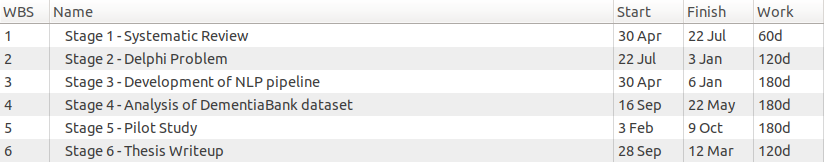
\includegraphics[width=400px, height=150px]{images/TasksAndDates.png}
\caption{Tasks and Dates}
\end{figure}

\subsection*{Stage 2 - Delphi Methodology and developing consensus on how best to collect language samples using technology}
The aim of this stage is to develop, in conjunction with experts, a convergence of ideas on how best to collect language samples using technology. The aim is to provide input from clinicians, technology experts and those using the technology within the homes to find the best protocol, and ideas for how to collect data with the focus on ease of use and non intrusiveness. The aim is to recruit no more than 20 participants with a rough guide of 5 clinicians, 5 technology experts and 10 users. Estimated completion, December 2019. This will form chapter 4 of my thesis and may produce a publication depending on the methodology used. 

\subsection*{Stage 3 - Development of a pipeline that processes language data accurately}
The aim of this stage is to build a data pipeline, and test the different technologies such as automated speech recognition software that might have an impact on the quality of the features generated. This is based on research done by Fraser (2015, 2019) who uses off the shelf products (Nuance - Dragon NaturallySpeaking) and open-source technology (Kaldi) as a means of converting speech to text. I would like to include tests of state of the art speech recognition from Google speech-to-text, IBM Watson and Amazon transcribe. This will also address the challenges unique to this population such as how to deal with changes in topic, hesitations, repetitions and so on. This will form chapter 5 of my thesis. The aim is to complete this by December 2019.

\subsection*{Stage 4 - Analysis of DementiaBank dataset, an exploration of existing and novel ways of classification of those with MCI and Early AD.}
The aim of this stage is to explore and identify language features that appear to be more important in the identification and classification of those with MCI and early AD. This stage will build upon the systematic review (stage 1) which, amongst other objectives, aims to identify language features other researchers have identified as useful in this problem. This stage will replicate and validate previous research results and introduce One Class Classification as a new way of classifying those with MCI and AD. This will form chapter 6 of my thesis. This should produce a publication. The aim is to complete this by March 2020.

\subsubsection*{One Class Classification}
The prevalence of Dementia in the UK's population is roughly 1 in 14 or 7\%. The prevalence of MCI has only briefly been explored, however some research by a team at the Univesity of Leeds indicate that the prevalence of MCI is between 3.2 - 24\%, and found that the prevalence of MCI in people who have self-reported memory problems is almost double (18\%) the amount of do not self report. Whilst this means that it is entirely possible to recruit a cohort with MCI and AD, it is comparatively costly in terms of time and resources. Given that, from a statistical perspective, this is a highly imbalanced population we can look at the problem as a kind of anomaly detection. This has some precedent in the field of Medicine, where examples of the 'positive' class can be costly or difficult to obtain. 
\par 
One-class classifiers analyse only examples of the majority class (in this case - Healthy Older Adults) to learn a classification boundary that excludes outlier examples. When dealing with heavily imbalanced datasets with text classification as an objective, the one-class classifier approach has been demonstrated to outperform conventional two-class classification.  

\subsection*{Stage 5 - Pilot study of the methodology developed}
The aim of this stage is to pilot the methodology developed in stage 2. Over a period of six months, 10 participants engage in collection of data and we analyse the results from both the participants perspective and the perspective of the researcher. From the participants perspective, we look at whether the process is comfortable and easy to use for the participant. From the researchers perspective, we look at the quality of the audio and whether there are any problems in the data pipeline. We also look at the quantity of language samples and whether the amount of language generated is enough for analysis. This will form chapter 7 of my thesis. This should produce a publication. The aim is to complete this by September 2020.

\begin{landscape}
\begin{figure}[H]
\centering
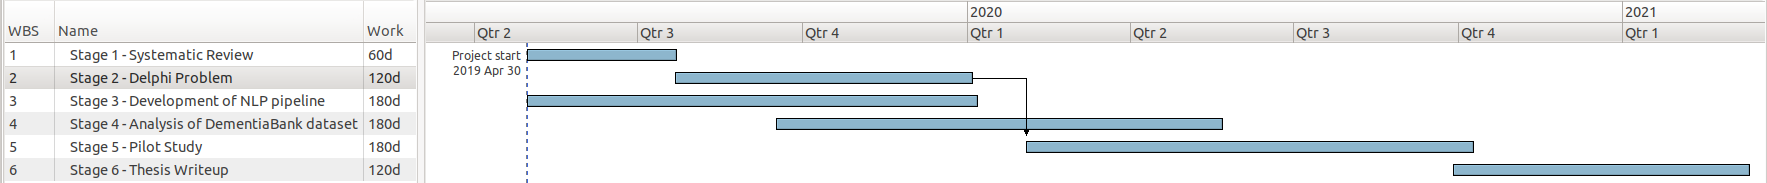
\includegraphics[width=650px, height=150px]{images/GanttChartUpdated.png}
\caption{Gantt Chart}
\end{figure}
\end{landscape}

\section{Use of additional resources}
It has been suggested that I potentially have the resource of a placement student from the Psychology department to help with my research. If this is still the case then I propose to get help with the following.

\begin{enumerate}
	\item Focus Groups - Conduct focus groups with various stakeholders as part of stage 2 (the adapted Delphi Methodology).
	\item Qualitative Analysis - Assist in the Qualitative Analysis of the transcripts / answers to the questions asked of the various stakeholders. 
	\item Recruitment - Recruitment into stage 5 (Pilot Study)
	\item Quantitative Analysis - Assist in the Analysis of the results of stage 5 (Pilot Study)
	\item Test Administration - Administration of any neuropsychological tests during stage 5 (Pilot Study)
	\item General research support - Responding to queries from stakeholders in stage 2 and pilot study participants in stage 5.
\end{enumerate}

\end{document}